% !TEX root = ../Survey.tex
\newpage
\section{Distance and related problems} \label{section:distance}
	The section begins in a rather broad literature review. 
	We then proceed to show the upper bound.
	A tight  connection between Distance, NCA in the fixed port model and separation level.
	We proceed by presenting  a revised lower bound.
	At this point we show results relating to approximate distance.
	After which we  show the dynamic labeling scheme by Korman.
	We finish the chapter by mentioning a close result of small distances in trees.
	
\subsection{Literature review}
	Distance labels were investigated at first by Peleg \cite{Peleg00}.
	Gavoille et al.~\cite{gavoillea2004distance,Gavoille2001} established a lower bound for $Trees(n)$.
		 Kano et. al~\cite{Kano07} present an average case analysis  for the function.
		Additional efforts by Kaplan \cite{Kaplan01} and Alstrup \cite{Alstrup05} showed a parameterized variant, where  the labeling scheme is limited to answer queries  up to some $k$. The first result presented a labeling scheme of  $\mathcal{O}(\log n + k \sqrt{\log n})$  \cite{Kaplan01}, and  improved  to $\log n+\mathcal{O}(k^2(\log \log n + \log k))$ \cite{Alstrup05}.	
		A well investigated variant are the approximate distance labeling schemes.
		Using $O(\log n \cdot \log \log n)$ bits Katz showed that an approximate scheme of $1+1 / log n$ stretch is possible.  The scheme still maintains distances for the separator at each level, using the first $\log \log n$ most significant bits \cite{Katz00} of each distance.The distance table of a tree with $n$ nodes can be distributed to each node, such that its label will contain all distances, which implies a labeling scheme of size $n \log n$.
		The immediate improvement is to store only the distance from each node to all its vertices on the path to the root. 
		The decoding will find the \emph{NCA} of both $u$ and $v$,$w$, and return $dist(u,w)+dist(v,w)$.
		Although better in practice, the maximum length of the labeling scheme remains $O(n \log n)$.
\subsection{Upper bound}
		The main question regarding the naive solution is, if there could be a smaller subset of distances to maintain in each label.
		For trees Peleg showed that it could be done with at most $\log n$ of those.
		Peleg considered  the weighted case with maximal weight $2^M$, and showed a  $O(M \log n + \log^2 n)$  distance labeling scheme, which yields a  $O(\log^2 n)$  distance labeling scheme for the unweighted case.		
		The result was re-discovered by Peleg as a private case of a graph separator related distance labeling scheme \cite{Gavoille2001}.
		
		\begin{lemma}\label{lemma:torwardsDistance}
		Given a tree $T=(V,E)$ with $n$ nodes, we can find a vertex $v \in V$ such that each of the $i$ connected components of $T \setminus v$ is a tree of size at most $\frac{n}{2}$.
		We denote vertex $v$ as the \emph{separator}  of $T$, and the components as $c_1 \dots c_i$ marked in a non decreasing order with respect to their size.
		\end{lemma}
		
		\begin{thm}\label{thm:distance-upper}
		There exist a distance labelling scheme for $Trees(n)$ with size at most $O(\log^2 n)$.
		\end{thm}
		\begin{notproof}
		Lemma~\ref{lemma:torwardsDistance} is  applied recursively such that it is guaranteed that after $\log n$ steps, each component consists of a single vertex.
		We denote for each $0 \leq j \leq \log n$  the $j$'th separator as $v_{s_j}$, and the components introduced as $c_1^j \dots c_i^j$.
		Each vertex is labeled by  a concatenation of $\log n$ tuples $ \tuple{d_j,c_i^j}, 0 \leq j \leq \log n $, where  $d_j$ is  the distance of the vertex from $v_{s_j}$.
		It can be shown that $\sum_{j=1}^{\log n}c_i^j=O(n)$, and since each $d_j=O(\log n)$ in the unweighted case,  the label size is $O(\log^2 n)$.
		The decoder finds the first uncommon connected component and returns the sum of distances from the separator thereof.
		\end{notproof}


\subsection{Lower bound for $Trees(n)$}
Gavoille et al.~\cite{gavoillea2004distance,Gavoille2001} establish a lower bound for $Trees(n)$ using a technique where they apply a distance labeling scheme to a special class of trees called $(h,M)$-trees. 
%proof has some errors and unclarities, which we shall try to fix in the following exposition. We shall later describe in more detail the problems with their proof.
\paragraph{$(h,M)$-trees}.
 For $h\geq 0$ and $M\geq 2$, an \emph{$(h,M)$-tree} is a binary tree that is constructed recursively as follows. 
 For $h=0$, the tree  a single node. For $h>0$, the tree consists of a path of length $M-x$ for some $0\leq x<M$ whose one end point is the root of the tree and whose other end point is the start node of two paths of length $x$ whose end points are the roots of two $(h-1,M)$-trees. An example for $h=3$ can be seen in  Fig.~\ref{fig:hMtree}.  We shall denote an $(h,M)$-tree constructed in this way by $T=\langle T_0,T_1,x\rangle$, where $T_0$ and $T_1$ are the two $(h-1,M)$-trees attached to the ends of the two paths of length $x$. Note that, if $x=0$, then the two paths of length $0$ collapse into a single node, and the two subtrees $T_0$ and $T_1$ are then both attached to this node.

\begin{figure}
	\centering
	\begin{tikzpicture}[sibling distance=3em, inner sep=0pt, minimum size=1ex]
	\tikzstyle{every node}=[draw,circle,fill=black]
	\Tree [.{} \edge node[draw=none,fill=none,auto=right] {$M-x$}; [.{} 
		\edge node[draw=none,fill=none,auto=right] {$x$}; [.{} \edge node[draw=none,fill=none,auto=right] {$M-y_1$}; [.{} 
			\edge node[draw=none,fill=none,auto=right] {$y_1$}; [.{} \edge node[draw=none,fill=none,draw=none,fill=none,auto=right] {$M-z_1$}; [.{} \edge node[draw=none,fill=none,auto=right,pos=.6] {$z_1$}; [ .{} ] \edge node[draw=none,fill=none,auto=left,pos=.6] {$z_1$}; [ .{} ] ] ]
			\edge node[draw=none,fill=none,auto=left] {$y_1$}; [.{} \edge node[draw=none,fill=none,auto=left] {$M-z_2$}; [.{} \edge node[draw=none,fill=none,auto=right,pos=.6] {$z_2$}; [ .{} ] \edge node[draw=none,fill=none,auto=left,pos=.6] {$z_2$}; [ .{} ] ] ]
			]
		]
		\edge node[draw=none,fill=none,auto=left] {$x$}; [.{}	\edge node[draw=none,fill=none,auto=left] {$M-y_2$}; [.{}
			\edge node[draw=none,fill=none,auto=right] {$y_2$}; [.{} \edge node[draw=none,fill=none,auto=right] {$M-z_3$}; [.{} \edge node[draw=none,fill=none,auto=right,pos=.6] {$z_3$}; [ .{} ] \edge node[draw=none,fill=none,auto=left,pos=.6] {$z_3$}; [ .{} ] ] ]
			\edge node[draw=none,fill=none,auto=left] {$y_2$}; [.{} \edge node[draw=none,fill=none,auto=left] {$M-z_4$}; [.{} \edge node[draw=none,fill=none,auto=right,pos=.6] {$z_4$}; [ .{} ] \edge node[draw=none,fill=none,auto=left,pos=.6] {$z_4$}; [ .{} ] ] ] 
			] 
		] 
	] ]
	\end{tikzpicture}
	\caption{An $(h,M)$-tree, where $h=3$. Each edge should be replaced by a path that is as long as the edge label indicates. If an edge label is $0$, then the two end nodes collapse into one single node.}
	\label{fig:hMtree}
\end{figure}


It is easy to see that %by induction that, if we keep the order of the nodes intact, there are $M^{2^h-1}$ distinct $(h,M)$-trees, each of which 
an $(h,M)$-tree
has at most $2^h$ leaves, at most $2^{h+1}M$ nodes in total and depth exactly equal to $hM$.  Further, it is straightforward to see that, if $u,v$ are leaves in an $(h,M)$-tree $T=\langle T_0,T_1,x\rangle$, then
\begin{equation} \label{eq:disthM}
\dist_T(u,v)= \begin{cases} 2(h-1)M + 2x,& \text{if $u\in T_0$ and $v\in T_1$, or vice versa,} \\ \dist_{T_i}(u,v), & \text{if $u,v\in T_i$ for some $i=0,1$}.\end{cases}
\end{equation}
%Thus, the distance between two nodes in an $(h,M)$-tree immediately reveal information about both the depth of the NCA of the two nodes as well as 

\paragraph{Leaf distance labeling schemes.}
In the following we shall consider \emph{leaf distance labeling schemes} for the family of $(h,M)$-trees: that is, distance labeling schemes where only the leaves in a tree need to be labeled, and where only leaf labels can be given as input to the decoder. Since an ordinary distance labeling scheme obviously can be used only for leaves, any lower bound on worst-case label sizes for a leaf distance labeling scheme is also a lower bound for an ordinary distance labeling scheme. We denote by $g(h,M)$ the smallest number of labels needed by an optimal leaf distance labeling scheme to label all $(h,M)$-trees.
\begin{lemma} \label{lemm:distancehM}
For all $h\geq 1$ and $M\geq 2$, $g(h,M)^2\geq Mg(h-1,M^2)$.
\end{lemma}
\begin{proof}
Let $h$ and $M$ be given, and fix an optimal leaf distance labeling scheme $\scheme$ which produces exactly $g(h,M)$ distinct labels for the family of $(h,M)$-trees. For leaves $u$ and $v$ in an $(h,M)$-tree, denote by $l(u)$ and $l(v)$, respectively, the labels assigned by the scheme $\scheme$. For $x=0,\dots ,M-1$, let $W(x)$ be the set consisting of pairs of labels $(l(u),l(v))$ for all leaves $u\in T_0$ and $v\in T_1$ in all $(h,M)$-trees $T=\langle T_0,T_1,x\rangle$.

The sets $W(x)$ and $W(x')$ are disjoint for $x\neq x'$, since every pair of labels in $W(x)$ uniquely determines $x$ because of the formula in~\eqref{eq:disthM}. Letting $W=\bigcup_{x=0}^{M-1}W(x)$, we therefore have $|W|=\sum_{x=0}^{M-1}|W(x)|$. 
Since $W$ contains pairs of labels produced by $\scheme$ from leaves in $(h,M)$-trees , we clearly also have $|W|\leq g(h,M)^2$, and hence it only remains to prove that $|W|\geq Mg(h-1,M^2)$, which we shall do by showing that $|W(x)|\geq g(h-1,M^2)$.

The goal for the rest of the proof is therefore to create a leaf distance labeling scheme for $(h-1,M^2)$-trees using only labels from the set $W(x)$ for some fixed $x$. So let $x$ be given and consider an $(h-1,M^2)$-tree $T'$. From $T'$ we shall construct an $(h-1,M)$-tree $\phi_i(T')$ for $i=0,1$ such that every leaf node $v$ in $T'$ corresponds to a node $\phi_i(v)$ in $\phi_i(T')$ for $i=0,1$.
The trees $\phi_i(T')$ are defined as follows.
If $h=1$, so that $T'$ consists of a single node, then $\phi_i(T')=T'$ for $i=0,1$. 
If $h>1$, then $T'$ is in the form $T'=\langle T'_0,T'_1,w\rangle$ for some $0\leq w< M^2$. We can write $w$ in the form $w=w_0+w_1M$ for uniquely determined $w_0,w_1$ with $0\leq w_0,w_1<M$. For $i=0,1$, we recursively define $\phi_i(T') = \langle \phi_i(T'_0), \phi_i(T'_1),w_i\rangle$. Thus, $\phi_i(T')$ is an $(h-1,M)$-tree that is similar to $T'$ but where we replace the two top paths of length $w$ by two paths of length $w_i$ and, recursively, do the same for all $(h-2,M^2)$-subtrees. Note also that the corresponding path of length $M^2-w$ in $T'$ automatically must be replaced by a path of length $M-w_i$ in $\phi_i(T')$ in order for $\phi_i(T')$ to be an $(h-1,M)$-tree.
Note that the number of leaves in $\phi_i(T')$ is less than or equal to the number of leaves in $T'$ (two leaves may collapse to one if $w>0$ and $w_i=0$), but no matter what, any leaf in $T'$ corresponds to a leaf in $\phi_i(T')$, namely the leaf at the end of the corresponding path. We denote by $\phi_i(v)$ the leaf in $\phi_i(T')$ corresponding to the leaf $v$ in $T'$.

Consider now the $(h,M)$-tree $T=\langle \phi_0(T'),\phi_1(T'),x\rangle$. Every leaf $v$ in $T'$ corresponds to the leaves $\phi_0(v),\phi_1(v)$ in $T$ where $\phi_i(v)\in \phi_i(T')$ for $i=0,1$. 
Using  formula~\eqref{eq:disthM} for the distances in $T'$, it is straightforward to see that
\begin{multline} \label{eq:disthMdistances}
\dist_{T'}(u,v) = \left(\dist_{\phi_0(T')}(\phi_0(u),\phi_0(v)) \bmod (2M)\right) \\
+ M\dist_{\phi_1(T')}(\phi_1(u),\phi_1(v)).
\end{multline}

We can now apply the leaf distance labeling scheme $\scheme$ to $T$ and obtain a label for each leaf node in $T$. In particular, the pair of leaves $(\phi_0(v),\phi_1(v))$ corresponding to a node $v$ in $T'$ will receive a pair of labels. We use this pair to label $v$ in $T'$, whereby we have obtained a labeling of the leaves in $T'$ with labels from $W(x)$. Using the formula in~\eqref{eq:disthMdistances} we can construct a decoder that can compute the distance between two nodes in $T'$ using these labels alone, and hence we have obtained a leaf distance labeling scheme for $(h-1,M^2)$-trees using only labels from $W(x)$ as desired.
\end{proof}

\begin{lemma} \label{lemm:distancehM2}
For all $h\geq 1$ and $M\geq 2$, $g(h,M)\geq M^{h/2}$.
\end{lemma}
\begin{proof}
The proof is by induction on $h$. For $h=1$ we note that an $(0,M)$-tree has only one node, so that $g(0,M^2)=1$. Lemma~\ref{lemm:distancehM} therefore yields $g(1,M)^2\geq M$ from which it follows that $g(1,M)\geq \sqrt{M}$. The claim therefore holds for $h=1$. Now let $h>1$ and assume that the claim holds for $h-1$. Lemma~\ref{lemm:distancehM} and the induction hypothesis now yields $g(h,M)^2\geq Mg(h-1,M^2)\geq M\cdot (M^2)^{(h-1)/2}=M^h$ from which it follows that $g(h,M)\geq M^{h/2}$.
\end{proof}

\begin{theorem} \label{theo:distancelowerbintrees}
For any $N\geq 8$, any distance labeling scheme for $\bintrees(N)$ has a worst-case label size of at least $\floor{\frac{1}{2}\floor{\frac{1}{2}(\log N-1)}^2}\geq\frac{1}{8}\log^2 N - \frac{3}{2}\log N$.
\end{theorem}
\begin{proof}
Set $n=2^{2\floor{\frac{1}{2}(\log N-1)}}$ be $N/2$ rounded down to the nearest even power of $2$, and set $h=\log \sqrt{n}$ and $M=\sqrt{n}$. Observe that $h$ and $M$ are both positive integers. Any $(h,M)$-tree has at most $2^{h+1} M = 2\sqrt{n}\sqrt{n}\leq N$ nodes and hence belongs to $\bintrees(N)$. A distance labeling scheme for $\bintrees(N)$ therefore induces a leaf distance labeling scheme for $(h,M)$-trees, and it follows from Lemma~\ref{lemm:distancehM2} that such a scheme must use at least $g(h,M)\geq M^{h/2}=n^{\frac{1}{8}\log n}$ labels. If the worst-case label size is $L$, we can create $2^{L+1}-1$ distinct labels, and we must therefore have $n^{\frac{1}{8}\log n}\leq 2^{L+1}-1$ from which it follows that $L\geq  \floor{\frac{1}{8}\log^2 n} = \floor{\frac{1}{2}\floor{\frac{1}{2}(\log N-1)}^2}$.
\end{proof}

We note that  the original proof of \ref{theo:distancelowerbintrees} by Gavoille et al.~\cite{gavoillea2004distance} contained a few problems. 
The construction of an $(h-1,M)$-tree from an $(h,M^2)$-tree (equivalent to \ref{lemm:distancehM}) is not, in fact, an $(h,M)$-tree since the corresponding weights (number of edges) do not add up to $M$.
An attempt to change  the  construction to make the weights (number of edges) add up to $M$, causes the  distance formula (equivalent to  \eqref{eq:disthMdistances}) to no longer holds.
Lastly,  the authors consider general labeling schemes and not just \emph{leaf} labeling schemes.
 Nonetheless, They only describe labels for the leaves without explaining how a leaf labeling scheme can be extended to a labeling scheme for the entire tree.


%\subsection{Approximate distance labeling scheme}
%		So far we have seen that to support exact distance labeling scheme, a label size of $O(log^2 n)$ is both possible and sufficient. 
%		Suppose  we now permit  our labeling scheme to return an approximation of the distance between the nodes, can we do better?
%		Gavoille, N. Katz, A. Katz, Paul and Peleg showed that $\log n \cdot O(\log \log n)$ are sufficient to determine a result which is 	at most $1/ \log n$ times larger than the real distance.
%		In fact, they showed that for such a factor, the label size is essentially tight.
%		The labeling scheme is based on the exact labeling scheme with the following alternation.
%		Rather than saving the distances from each vertex to the set of all separators in its connected component, the authors used the $2$-approx. trick and save distances from each separator.
%		
%
%
%		Recall that for any two nodes $u, v \in T$ where $T$ is a tree rooted in $r$ is , $\dist(u,v) = \dist(u,NCA(u,v))+\dist(v,NCA(u,v))$.
%		An alternative way to compute distance is the following.
%		 $$\dist(u,v) = \dist(r,u)+\dist(t,v) - 2 \dist(r,NCA(u,v))$$
%		 
%		 In addition, recall that there exist an $O(\log n)$ NCA  labeling scheme for $Trees$  such that $\la(v) = h_1(v),l_1(v) \dots h_k(v),l_k(v)$ for every node $v \in T$ with $1 \leq k \leq \log $ light nodes. 
%		 
%		\begin{open}
%		Does there exist a $1+ 1/\epsilon$ approximate distance labeling scheme with labels of size at most $O(\log n \cdot \epsilon)$?
%		\end{open}


%\subsection{Small distances}\label{section:Sma}
%Recall that there exist an adjacency labeling scheme of size $\log n +O(\log^*n)$. For unbounded distance queries Theorem~\ref{theo:distancelowerbintrees} showed a lower bound of $\Omega(\log^2(n))$.
%A follow up question is to find out what is the label size required, or possible, for a limited distance query.
%By that we mean a distance query built to return distances up to a constant $k$, and infinity if the distance is larger than that.
%Alstrup, Bille and Rauhe~\cite{Alstrup05} (Section 3.2) showed, that such a query in fact  require and have  a label of an intermediate size.
%\begin{thm}
%There exist a $k-Small-Distance$ labeling scheme $Trees(n)$ with label size bounded by $\log n + O(k^2(\log \log n +\log k))$.
%\end{thm}
%\begin{notproof}
%We describe the encoder operation on a tree $T \in  Trees(n)$.
%The encoder builds on the adjacency labeling scheme present in Lemma~\ref{Lemma-adj-loglogn}.
%The idea is to store, for every vertex $v \in V$ $pre(v)$, $lightdepth(v)$, and an \emph{ancestor table} of the number of significant ancestor of distance at most $k$ from $v$.
%Each of those of size $O(k \log \log n = k \log k)$.
%
%\end{notproof}
%Gavoille and Labourel~\cite{gavoille07} later improved the label size for the query on the expanse of slower encoder.
%\begin{thm}
%
%\end{thm}
%\begin{notproof}
%\end{notproof}


